%% bare_jrnl.tex
%% V1.4
%% 2012/12/27
%% by Michael Shell
%% see http://www.michaelshell.org/
%% for current contact information.
%%
%% updated by Trevor Tomesh
%% trevortomesh.github.io
%% 2019/01/16
%% trevor.tomesh@uregina.ca
%%
%% This is a skeleton file demonstrating the use of IEEEtran.cls
%%
%% (requires IEEEtran.cls version 1.8 or later) with an IEEE journal paper.
%%
%% Support sites:
%% http://www.michaelshell.org/tex/ieeetran/
%% http://www.ctan.org/tex-archive/macros/latex/contrib/IEEEtran/
%% and
%% http://www.ieee.org/

% *** Authors should verify (and, if needed, correct) their LaTeX system  ***
% *** with the testflow diagnostic prior to trusting their LaTeX platform ***
% *** with production work. IEEE's font choices can trigger bugs that do  ***
% *** not appear when using other class files.                            ***
% The testflow support page is at:
% http://www.michaelshell.org/tex/testflow/

%%*************************************************************************
%% Legal Notice:
%% This code is offered as-is without any warranty either expressed or
%% implied; without even the implied warranty of MERCHANTABILITY or
%% FITNESS FOR A PARTICULAR PURPOSE! 
%% User assumes all risk.
%% In no event shall IEEE or any contributor to this code be liable for
%% any damages or losses, including, but not limited to, incidental,
%% consequential, or any other damages, resulting from the use or misuse
%% of any information contained here.
%%
%% All comments are the opinions of their respective authors and are not
%% necessarily endorsed by the IEEE.
%%
%% This work is distributed under the LaTeX Project Public License (LPPL)
%% ( http://www.latex-project.org/ ) version 1.3, and may be freely used,
%% distributed and modified. A copy of the LPPL, version 1.3, is included
%% in the base LaTeX documentation of all distributions of LaTeX released
%% 2003/12/01 or later.
%% Retain all contribution notices and credits.
%% ** Modified files should be clearly indicated as such, including  **
%% ** renaming them and changing author support contact information. **
%%
%% File list of work: IEEEtran.cls, IEEEtran_HOWTO.pdf, bare_adv.tex,
%%                    bare_conf.tex, bare_jrnl.tex, bare_jrnl_compsoc.tex,
%%                    bare_jrnl_transmag.tex
%%*************************************************************************

% Note that the a4paper option is mainly intended so that authors in
% countries using A4 can easily print to A4 and see how their papers will
% look in print - the typesetting of the document will not typically be
% affected with changes in paper size (but the bottom and side margins will).
% Use the testflow package mentioned above to verify correct handling of
% both paper sizes by the user's LaTeX system.
%
% Also note that the "draftcls" or "draftclsnofoot", not "draft", option
% should be used if it is desired that the figures are to be displayed in
% draft mode.
%
\documentclass[journal]{IEEEtran}
%
% If IEEEtran.cls has not been installed into the LaTeX system files,
% manually specify the path to it like:
% \documentclass[journal]{../sty/IEEEtran} 



% Some very useful LaTeX packages include:
% (uncomment the ones you want to load)


% *** MISC UTILITY PACKAGES ***
%
%\usepackage{ifpdf}
% Heiko Oberdiek's ifpdf.sty is very useful if you need conditional
% compilation based on whether the output is pdf or dvi.
% usage:
% \ifpdf
%   % pdf code
% \else
%   % dvi code
% \fi
% The latest version of ifpdf.sty can be obtained from:
% http://www.ctan.org/tex-archive/macros/latex/contrib/oberdiek/
% Also, note that IEEEtran.cls V1.7 and later provides a builtin
% \ifCLASSINFOpdf conditional that works the same way.
% When switching from latex to pdflatex and vice-versa, the compiler may
% have to be run twice to clear warning/error messages.






% *** CITATION PACKAGES ***
%
%\usepackage{cite}
% cite.sty was written by Donald Arseneau
% V1.6 and later of IEEEtran pre-defines the format of the cite.sty package
% \cite{} output to follow that of IEEE. Loading the cite package will
% result in citation numbers being automatically sorted and properly
% "compressed/ranged". e.g., [1], [9], [2], [7], [5], [6] without using
% cite.sty will become [1], [2], [5]--[7], [9] using cite.sty. cite.sty's
% \cite will automatically add leading space, if needed. Use cite.sty's
% noadjust option (cite.sty V3.8 and later) if you want to turn this off
% such as if a citation ever needs to be enclosed in parenthesis.
% cite.sty is already installed on most LaTeX systems. Be sure and use
% version 4.0 (2003-05-27) and later if using hyperref.sty. cite.sty does
% not currently provide for hyperlinked citations.
% The latest version can be obtained at:
% http://www.ctan.org/tex-archive/macros/latex/contrib/cite/
% The documentation is contained in the cite.sty file itself.






% *** GRAPHICS RELATED PACKAGES ***
%

\usepackage{graphicx}
\usepackage{placeins}
\graphicspath{ {./img/} }

\ifCLASSINFOpdf
  % \usepackage[pdftex]{graphicx}
  % declare the path(s) where your graphic files are
  % \graphicspath{{../pdf/}{../jpeg/}}
  % and their extensions so you won't have to specify these with
  % every instance of \includegraphics
  % \DeclareGraphicsExtensions{.pdf,.jpeg,.png}
\else
  % or other class option (dvipsone, dvipdf, if not using dvips). graphicx
  % will default to the driver specified in the system graphics.cfg if no
  % driver is specified.
  % \usepackage[dvips]{graphicx}
  % declare the path(s) where your graphic files are
  % \graphicspath{{../eps/}}
  % and their extensions so you won't have to specify these with
  % every instance of \includegraphics
  % \DeclareGraphicsExtensions{.eps}
\fi
% graphicx was written by David Carlisle and Sebastian Rahtz. It is
% required if you want graphics, photos, etc. graphicx.sty is already
% installed on most LaTeX systems. The latest version and documentation
% can be obtained at: 
% http://www.ctan.org/tex-archive/macros/latex/required/graphics/
% Another good source of documentation is "Using Imported Graphics in
% LaTeX2e" by Keith Reckdahl which can be found at:
% http://www.ctan.org/tex-archive/info/epslatex/
%
% latex, and pdflatex in dvi mode, support graphics in encapsulated
% postscript (.eps) format. pdflatex in pdf mode supports graphics
% in .pdf, .jpeg, .png and .mps (metapost) formats. Users should ensure
% that all non-photo figures use a vector format (.eps, .pdf, .mps) and
% not a bitmapped formats (.jpeg, .png). IEEE frowns on bitmapped formats
% which can result in "jaggedy"/blurry rendering of lines and letters as
% well as large increases in file sizes.
%
% You can find documentation about the pdfTeX application at:
% http://www.tug.org/applications/pdftex





% *** MATH PACKAGES ***
%
%\usepackage[cmex10]{amsmath}
% A popular package from the American Mathematical Society that provides
% many useful and powerful commands for dealing with mathematics. If using
% it, be sure to load this package with the cmex10 option to ensure that
% only type 1 fonts will utilized at all point sizes. Without this option,
% it is possible that some math symbols, particularly those within
% footnotes, will be rendered in bitmap form which will result in a
% document that can not be IEEE Xplore compliant!
%
% Also, note that the amsmath package sets \interdisplaylinepenalty to 10000
% thus preventing page breaks from occurring within multiline equations. Use:
%\interdisplaylinepenalty=2500
% after loading amsmath to restore such page breaks as IEEEtran.cls normally
% does. amsmath.sty is already installed on most LaTeX systems. The latest
% version and documentation can be obtained at:
% http://www.ctan.org/tex-archive/macros/latex/required/amslatex/math/





% *** SPECIALIZED LIST PACKAGES ***
%
%\usepackage{algorithmic}
% algorithmic.sty was written by Peter Williams and Rogerio Brito.
% This package provides an algorithmic environment fo describing algorithms.
% You can use the algorithmic environment in-text or within a figure
% environment to provide for a floating algorithm. Do NOT use the algorithm
% floating environment provided by algorithm.sty (by the same authors) or
% algorithm2e.sty (by Christophe Fiorio) as IEEE does not use dedicated
% algorithm float types and packages that provide these will not provide
% correct IEEE style captions. The latest version and documentation of
% algorithmic.sty can be obtained at:
% http://www.ctan.org/tex-archive/macros/latex/contrib/algorithms/
% There is also a support site at:
% http://algorithms.berlios.de/index.html
% Also of interest may be the (relatively newer and more customizable)
% algorithmicx.sty package by Szasz Janos:
% http://www.ctan.org/tex-archive/macros/latex/contrib/algorithmicx/




% *** ALIGNMENT PACKAGES ***
%
%\usepackage{array}
% Frank Mittelbach's and David Carlisle's array.sty patches and improves
% the standard LaTeX2e array and tabular environments to provide better
% appearance and additional user controls. As the default LaTeX2e table
% generation code is lacking to the point of almost being broken with
% respect to the quality of the end results, all users are strongly
% advised to use an enhanced (at the very least that provided by array.sty)
% set of table tools. array.sty is already installed on most systems. The
% latest version and documentation can be obtained at:
% http://www.ctan.org/tex-archive/macros/latex/required/tools/


% IEEEtran contains the IEEEeqnarray family of commands that can be used to
% generate multiline equations as well as matrices, tables, etc., of high
% quality.




% *** SUBFIGURE PACKAGES ***
%\ifCLASSOPTIONcompsoc
%  \usepackage[caption=false,font=normalsize,labelfont=sf,textfont=sf]{subfig}
%\else
%  \usepackage[caption=false,font=footnotesize]{subfig}
%\fi
% subfig.sty, written by Steven Douglas Cochran, is the modern replacement
% for subfigure.sty, the latter of which is no longer maintained and is
% incompatible with some LaTeX packages including fixltx2e. However,
% subfig.sty requires and automatically loads Axel Sommerfeldt's caption.sty
% which will override IEEEtran.cls' handling of captions and this will result
% in non-IEEE style figure/table captions. To prevent this problem, be sure
% and invoke subfig.sty's "caption=false" package option (available since
% subfig.sty version 1.3, 2005/06/28) as this is will preserve IEEEtran.cls
% handling of captions.
% Note that the Computer Society format requires a larger sans serif font
% than the serif footnote size font used in traditional IEEE formatting
% and thus the need to invoke different subfig.sty package options depending
% on whether compsoc mode has been enabled.
%
% The latest version and documentation of subfig.sty can be obtained at:
% http://www.ctan.org/tex-archive/macros/latex/contrib/subfig/




% *** FLOAT PACKAGES ***
%
%\usepackage{fixltx2e}
% fixltx2e, the successor to the earlier fix2col.sty, was written by
% Frank Mittelbach and David Carlisle. This package corrects a few problems
% in the LaTeX2e kernel, the most notable of which is that in current
% LaTeX2e releases, the ordering of single and double column floats is not
% guaranteed to be preserved. Thus, an unpatched LaTeX2e can allow a
% single column figure to be placed prior to an earlier double column
% figure. The latest version and documentation can be found at:
% http://www.ctan.org/tex-archive/macros/latex/base/


%\usepackage{stfloats}
% stfloats.sty was written by Sigitas Tolusis. This package gives LaTeX2e
% the ability to do double column floats at the bottom of the page as well
% as the top. (e.g., "\begin{figure*}[!b]" is not normally possible in
% LaTeX2e). It also provides a command:
%\fnbelowfloat
% to enable the placement of footnotes below bottom floats (the standard
% LaTeX2e kernel puts them above bottom floats). This is an invasive package
% which rewrites many portions of the LaTeX2e float routines. It may not work
% with other packages that modify the LaTeX2e float routines. The latest
% version and documentation can be obtained at:
% http://www.ctan.org/tex-archive/macros/latex/contrib/sttools/
% Do not use the stfloats baselinefloat ability as IEEE does not allow
% \baselineskip to stretch. Authors submitting work to the IEEE should note
% that IEEE rarely uses double column equations and that authors should try
% to avoid such use. Do not be tempted to use the cuted.sty or midfloat.sty
% packages (also by Sigitas Tolusis) as IEEE does not format its papers in
% such ways.
% Do not attempt to use stfloats with fixltx2e as they are incompatible.
% Instead, use Morten Hogholm'a dblfloatfix which combines the features
% of both fixltx2e and stfloats:
%
% \usepackage{dblfloatfix}
% The latest version can be found at:
% http://www.ctan.org/tex-archive/macros/latex/contrib/dblfloatfix/




%\ifCLASSOPTIONcaptionsoff
%  \usepackage[nomarkers]{endfloat}
% \let\MYoriglatexcaption\caption
% \renewcommand{\caption}[2][\relax]{\MYoriglatexcaption[#2]{#2}}
%\fi
% endfloat.sty was written by James Darrell McCauley, Jeff Goldberg and 
% Axel Sommerfeldt. This package may be useful when used in conjunction with 
% IEEEtran.cls'  captionsoff option. Some IEEE journals/societies require that
% submissions have lists of figures/tables at the end of the paper and that
% figures/tables without any captions are placed on a page by themselves at
% the end of the document. If needed, the draftcls IEEEtran class option or
% \CLASSINPUTbaselinestretch interface can be used to increase the line
% spacing as well. Be sure and use the nomarkers option of endfloat to
% prevent endfloat from "marking" where the figures would have been placed
% in the text. The two hack lines of code above are a slight modification of
% that suggested by in the endfloat docs (section 8.4.1) to ensure that
% the full captions always appear in the list of figures/tables - even if
% the user used the short optional argument of \caption[]{}.
% IEEE papers do not typically make use of \caption[]'s optional argument,
% so this should not be an issue. A similar trick can be used to disable
% captions of packages such as subfig.sty that lack options to turn off
% the subcaptions:
% For subfig.sty:
% \let\MYorigsubfloat\subfloat
% \renewcommand{\subfloat}[2][\relax]{\MYorigsubfloat[]{#2}}
% However, the above trick will not work if both optional arguments of
% the \subfloat command are used. Furthermore, there needs to be a
% description of each subfigure *somewhere* and endfloat does not add
% subfigure captions to its list of figures. Thus, the best approach is to
% avoid the use of subfigure captions (many IEEE journals avoid them anyway)
% and instead reference/explain all the subfigures within the main caption.
% The latest version of endfloat.sty and its documentation can obtained at:
% http://www.ctan.org/tex-archive/macros/latex/contrib/endfloat/
%
% The IEEEtran \ifCLASSOPTIONcaptionsoff conditional can also be used
% later in the document, say, to conditionally put the References on a 
% page by themselves.




% *** PDF, URL AND HYPERLINK PACKAGES ***
%
%\usepackage{url}
% url.sty was written by Donald Arseneau. It provides better support for
% handling and breaking URLs. url.sty is already installed on most LaTeX
% systems. The latest version and documentation can be obtained at:
% http://www.ctan.org/tex-archive/macros/latex/contrib/url/
% Basically, \url{my_url_here}.




% *** Do not adjust lengths that control margins, column widths, etc. ***
% *** Do not use packages that alter fonts (such as pslatex).         ***
% There should be no need to do such things with IEEEtran.cls V1.6 and later.
% (Unless specifically asked to do so by the journal or conference you plan
% to submit to, of course. )


% correct bad hyphenation here
\hyphenation{op-tical net-works semi-conduc-tor}


\begin{document}

% paper title
% can use linebreaks \\ within to get better formatting as desired
% Do not put math or special symbols in the title.

\title{Teardown of PEAK\textsuperscript{TM} PKCORJ GARAGE PARKING SENSOR}


\author{Trevor~Tomesh,~\IEEEmembership{Sessional Lecturer,~University~of~Regina}
        %other authors go below
        %Bob~Builder,~\IEEEmembership{Student,~University~of~Regina,}
        %and~Noob~McScrubb,~\IEEEmembership{Student,~University~of~Regina}
        }


% The paper headers
\markboth{CS807~Interactive~Hardware, Jan~17th~2019}%
{Shell \MakeLowercase{\textit{et al.}}: Design, Template, Computer Science }
% The only time the second header will appear is for the odd numbered pages
% after the title page when using the twoside option.


% make the title area
\maketitle

% As a general rule, do not put math, special symbols or citations
% in the abstract or keywords.
\begin{abstract}
In this document we describe the teardown process of a PEAK\textsuperscript{TM} PKCORJ GARAGE PARKING SENSOR. 
We detail the advertised function of the device, discuss the process of opening and removing the various 
components from the shell and describe various components that are of interest. Furthermore, we discuss some
of the more novel design decisions observed and how some of the components and design decisions may be appropriated
for future projects. 


\end{abstract}

% Note that keywords are not normally used for peerreview papers.
\begin{IEEEkeywords}
teardown, electronics, sensor, design
\end{IEEEkeywords}

% For peer review papers, you can put extra information on the cover
% page as needed:
% \ifCLASSOPTIONpeerreview
% \begin{center} \bfseries EDICS Category: 3-BBND \end{center}
% \fi
%
% For peerreview papers, this IEEEtran command inserts a page break and
% creates the second title. It will be ignored for other modes.

\IEEEpeerreviewmaketitle

\section{Introduction}
% The very first letter is a 2 line initial drop letter followed
% by the rest of the first word in caps.
% 
% form to use if the first word consists of a single letter:
% \IEEEPARstart{A}{demo} file is ....
% 
% form to use if you need the single drop letter followed by
% normal text (unknown if ever used by IEEE):
% \IEEEPARstart{A}{}demo file is ....
% 
% Some journals put the first two words in caps:
% \IEEEPARstart{T}{his demo} file is ....
% 
% Here we have the typical use of a "T" for an initial drop letter
% and "HIS" in caps to complete the first word.
\IEEEPARstart{T}{he} PEAK\textsuperscript{TM} PKCORJ GARAGE PARKING SENSOR is advertised per the packaging as an 
``easy to install and use'' solution to ``safely park your vehicle every time.'' The sensor was purchased at a local 
DOLLARAMA for 4 CAD. The device is intended for use in personal garages. An ultrasonic sensor attached to the main device detects the distance of any object in front of it -- presumably a vehicle -- and gives feedback in the form of a glowing light which changes color 
depending upon how close an object is. According to the packaging, the sensor will turn green if the object is within 4-8 feet, 
yellow if it is between 2-4 feet and red if it is between 0-2 feet. According to the packaging, the system is also 
programmable via a ``learn'' button which allows the user to define the optimal distance from the sensor. While the packaging 
originally came with a detailed manual for the device, it has long been lost and all attempts at recovering the manual online 
have failed. 
% You must have at least 2 lines in the paragraph with the drop letter
% (should never be an issue)

\section{Motivation}
The motivation for this teardown was simply to see what sort of components are inside of it, to document 
the internals and to find potentially salvageable parts for use in future projects. The form factor of 
the device in-packaging looked like a promising source of modular components. Moreover, it is the experience
of the author that electronic devices purchased from the DOLLARAMA tend to be built as inexpensively as possible 
and hence the designs often rely on stock through-hole components that are accessible for repurposing as opposed
to difficult-to-remove surface mounted devices.   

\section{Required Tools}
The only tools required for this teardown was Phillips size 1 screwdriver.

\section{Teardown Process and Description}
\subsection{Opening the Shell}
The teardown process was fairly straightforward. There are four screws on the back of the device that serve to 
hold the back of the shell to the front. Once removed, the shell comes apart with very little effort. 

\begin{figure}[h]
  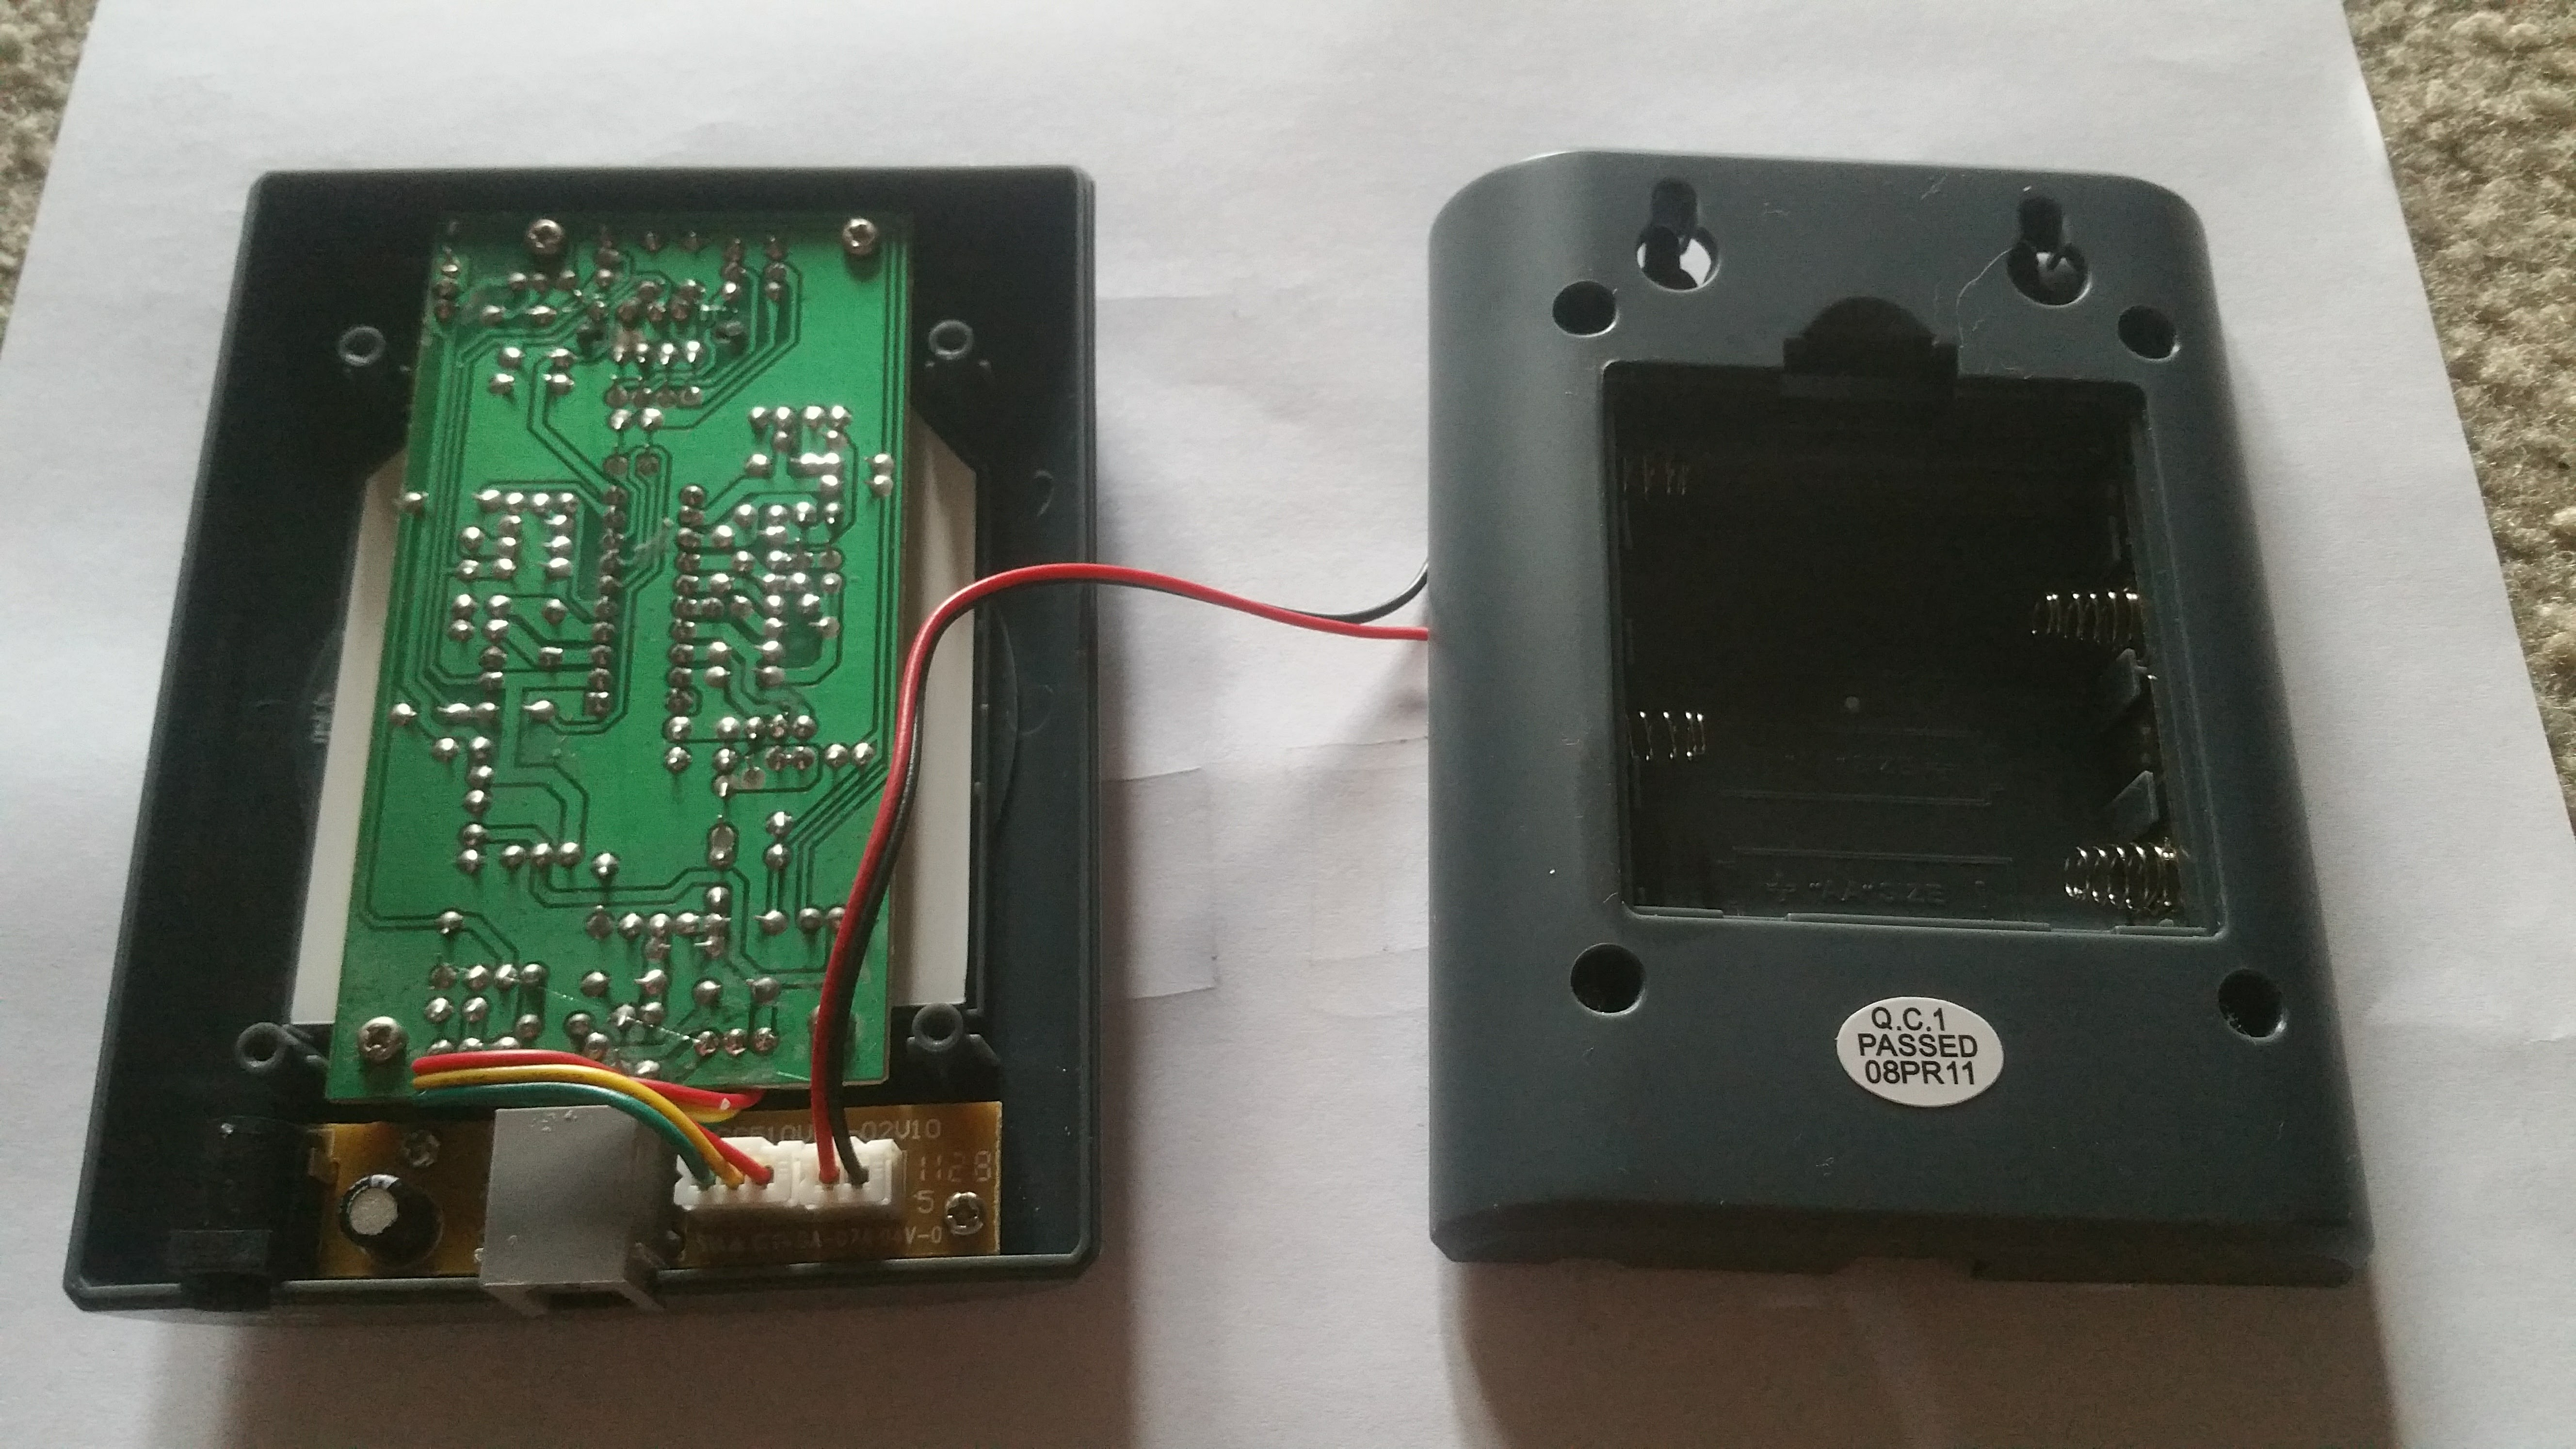
\includegraphics[width=0.5\textwidth]{img/img4.jpg}
  \caption{The parking sensor once the screws have been removed revealing the primary printed circuit board}
  \label{fig:img4}
\end{figure}

As is evident in Fig. \ref{fig:img4}, the front and the back portions of the shells are connected to one another via a
two-wire plug. This plug serves as the connection between the battery bank (on the right) and the rest of the circuitry 
(on the left). Two distinct printed circuit boards are visible. The smaller one in the lower-left portion of Fig. \ref{fig:img4}
connects to both the main printed circuit board and the the ultrasonic sensor (not pictured). In the lower left-hand section
of Fig. \ref{fig:img4}, the jack for an external power supply is present along with a capacitor. 

\subsection{The Main Printed Circuit Board}
To free the main PCB, four screws -- one on each corner -- must be removed. The PCB must also be unplugged from the 
secondary PCB as it is connected via a three-wire (red, yellow, green) plug. On the side opposite the traces there are a number 
of components as can be seen in Fig. \ref{fig:img6}. These components are:
\begin{itemize}
  \item{HT46R503 2K 8-Bit OTP MCU with OPA and Comparator \cite{holtek:holtek}}
  \item{8 KHz Oscillator}
  \item{7 transistors:}
  \begin{itemize}
    \item{S8050}
    \item{S8550}
    \item{S9104}
    \item{S9014 x 4}
  \end{itemize}  
 \item{7039A-1 Low Power Detector}
 \item{7333A Low power high voltage regulators}  
 \item{Various Capacitors between 0.0001 $\mu$F and 220 $\mu$F}
 \item {Various Resistors}
\end{itemize}

\begin{figure}[h]
  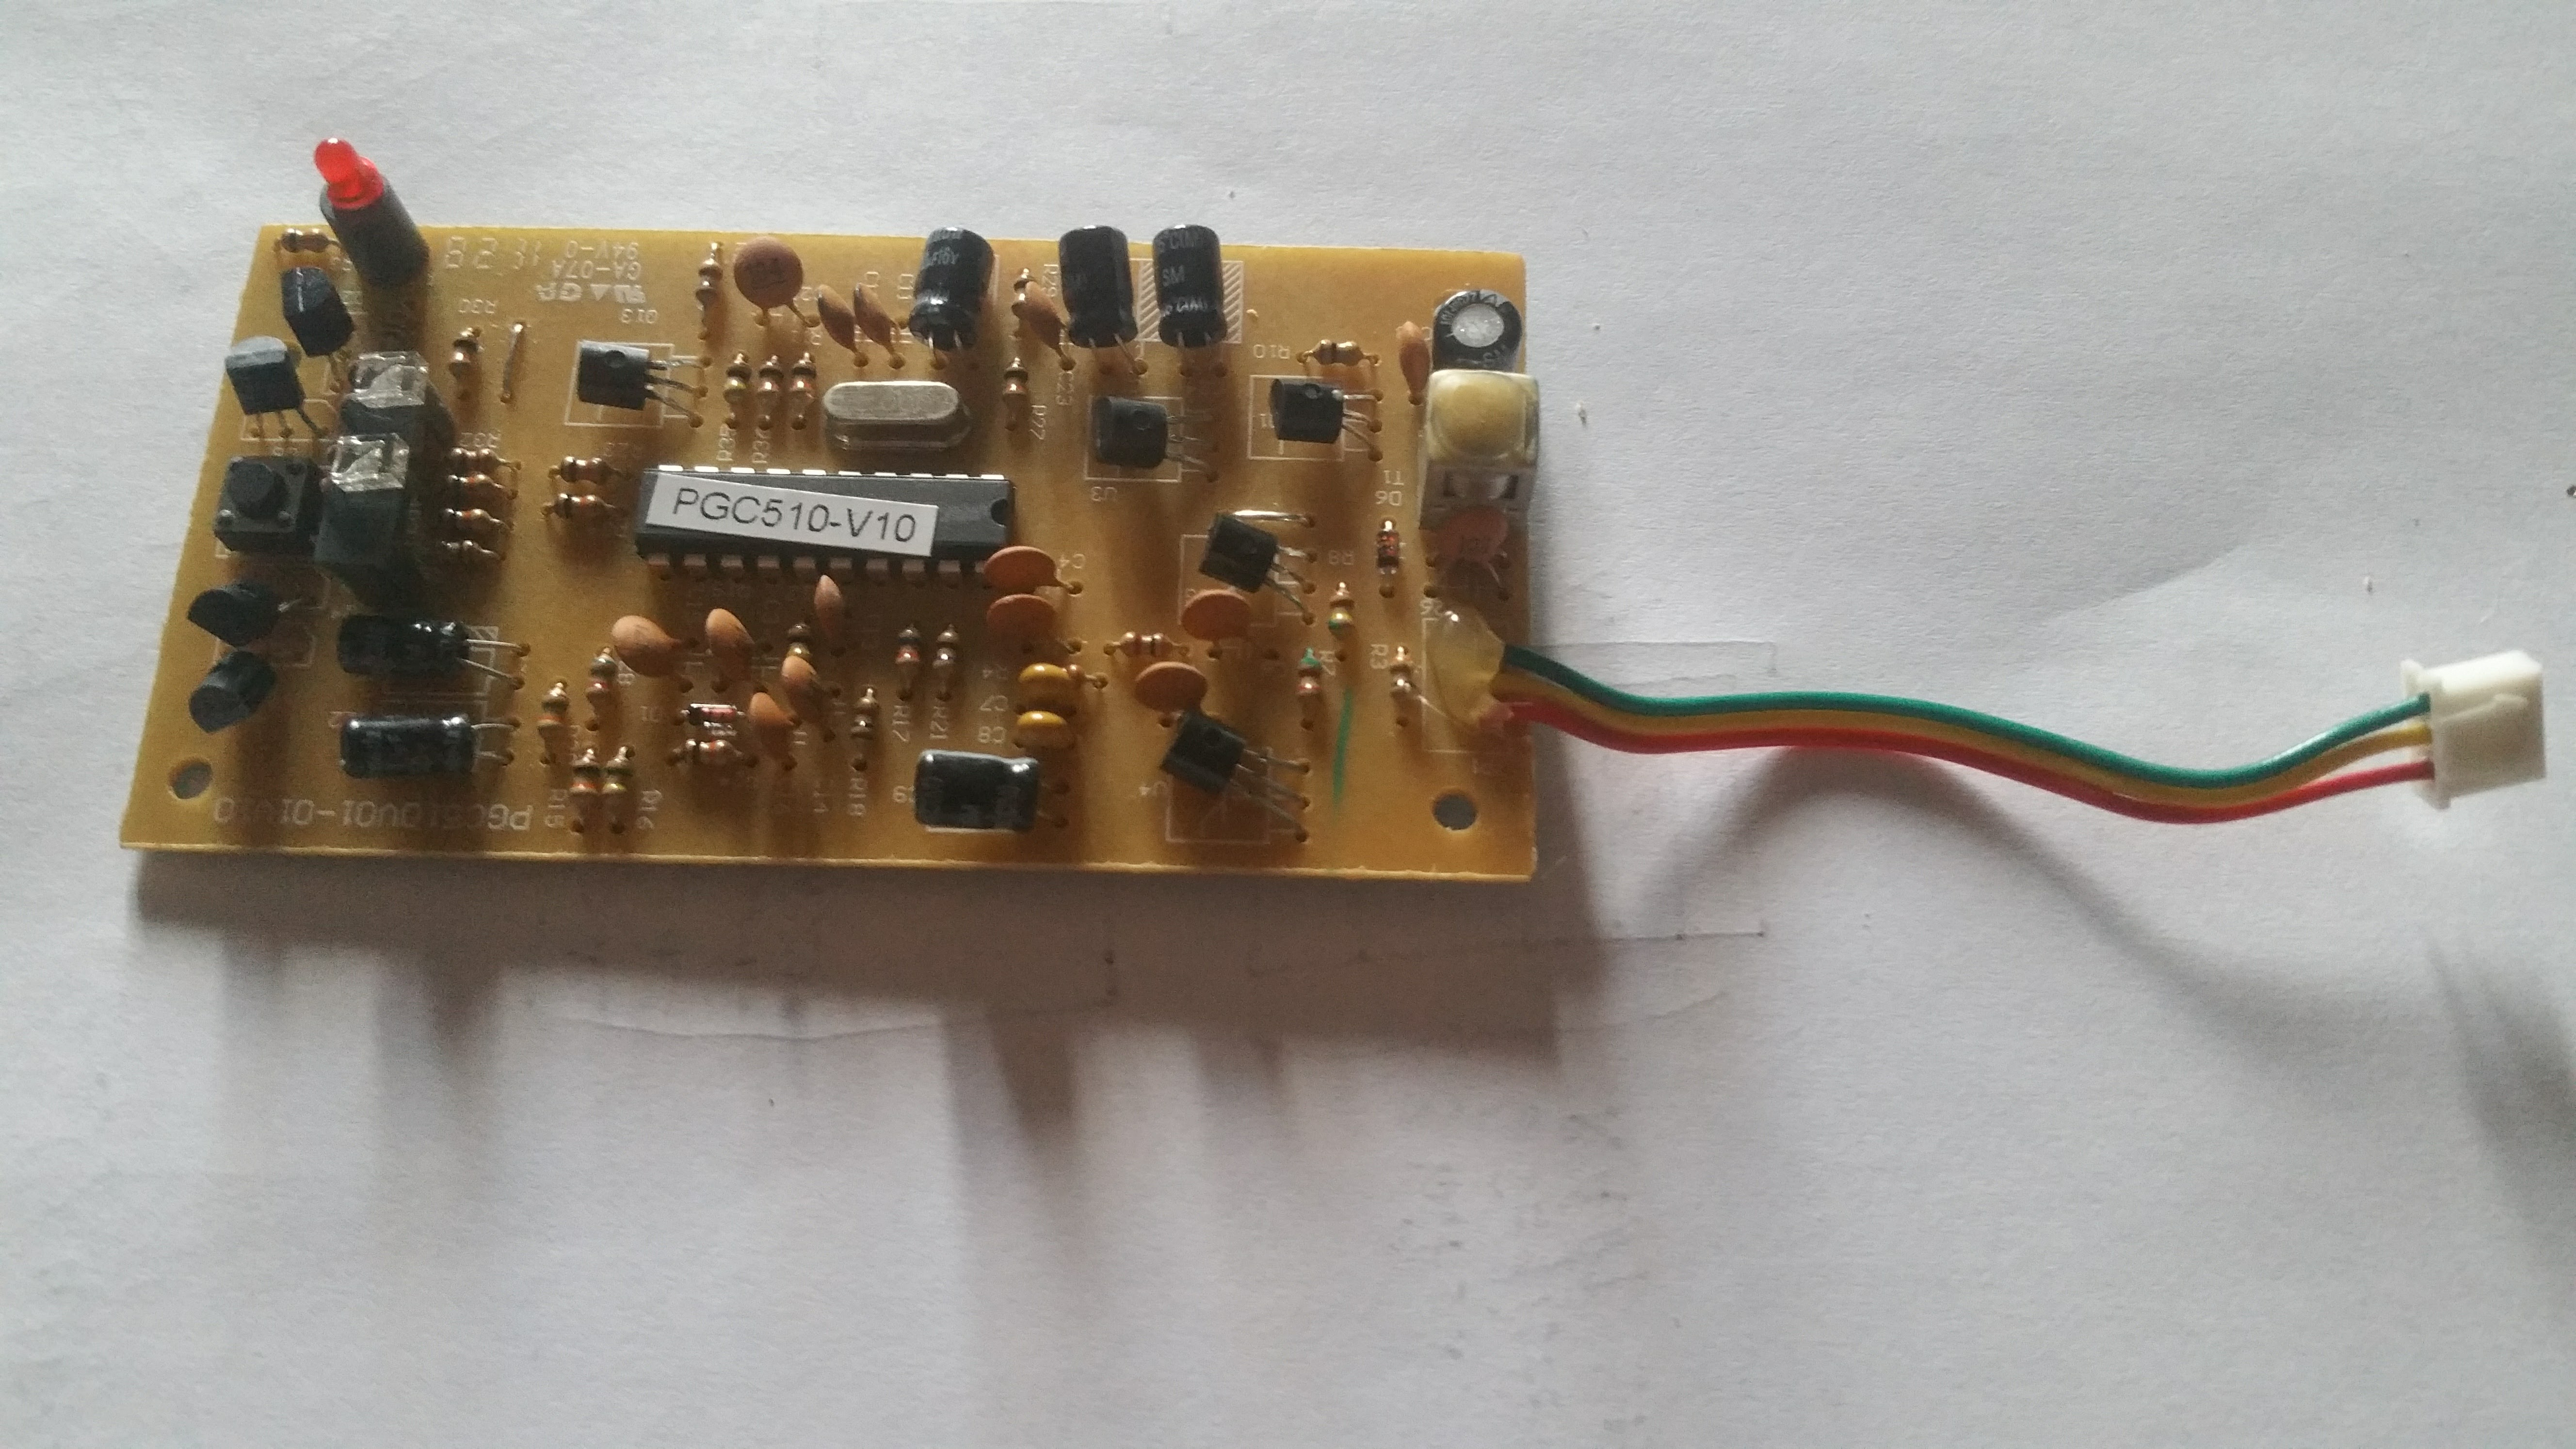
\includegraphics[width=0.5\textwidth]{img/img6.jpg}
  \caption{The primary printed circuit board with components visible}
  \label{fig:img6}
\end{figure}

\subsection{The Secondary Printed Circuit Board}
The secondary circuit board, pictured in Fig. \ref{fig:img8}, is removed with two standard Phillips screws. This board contains a single capacitor, a power jack for external power, a two-pronged plug to connect to the battery pack, a three-pronged 
plug to connect to the main board, and a patch cable which connects to the sensor. 

\begin{figure}[h]
  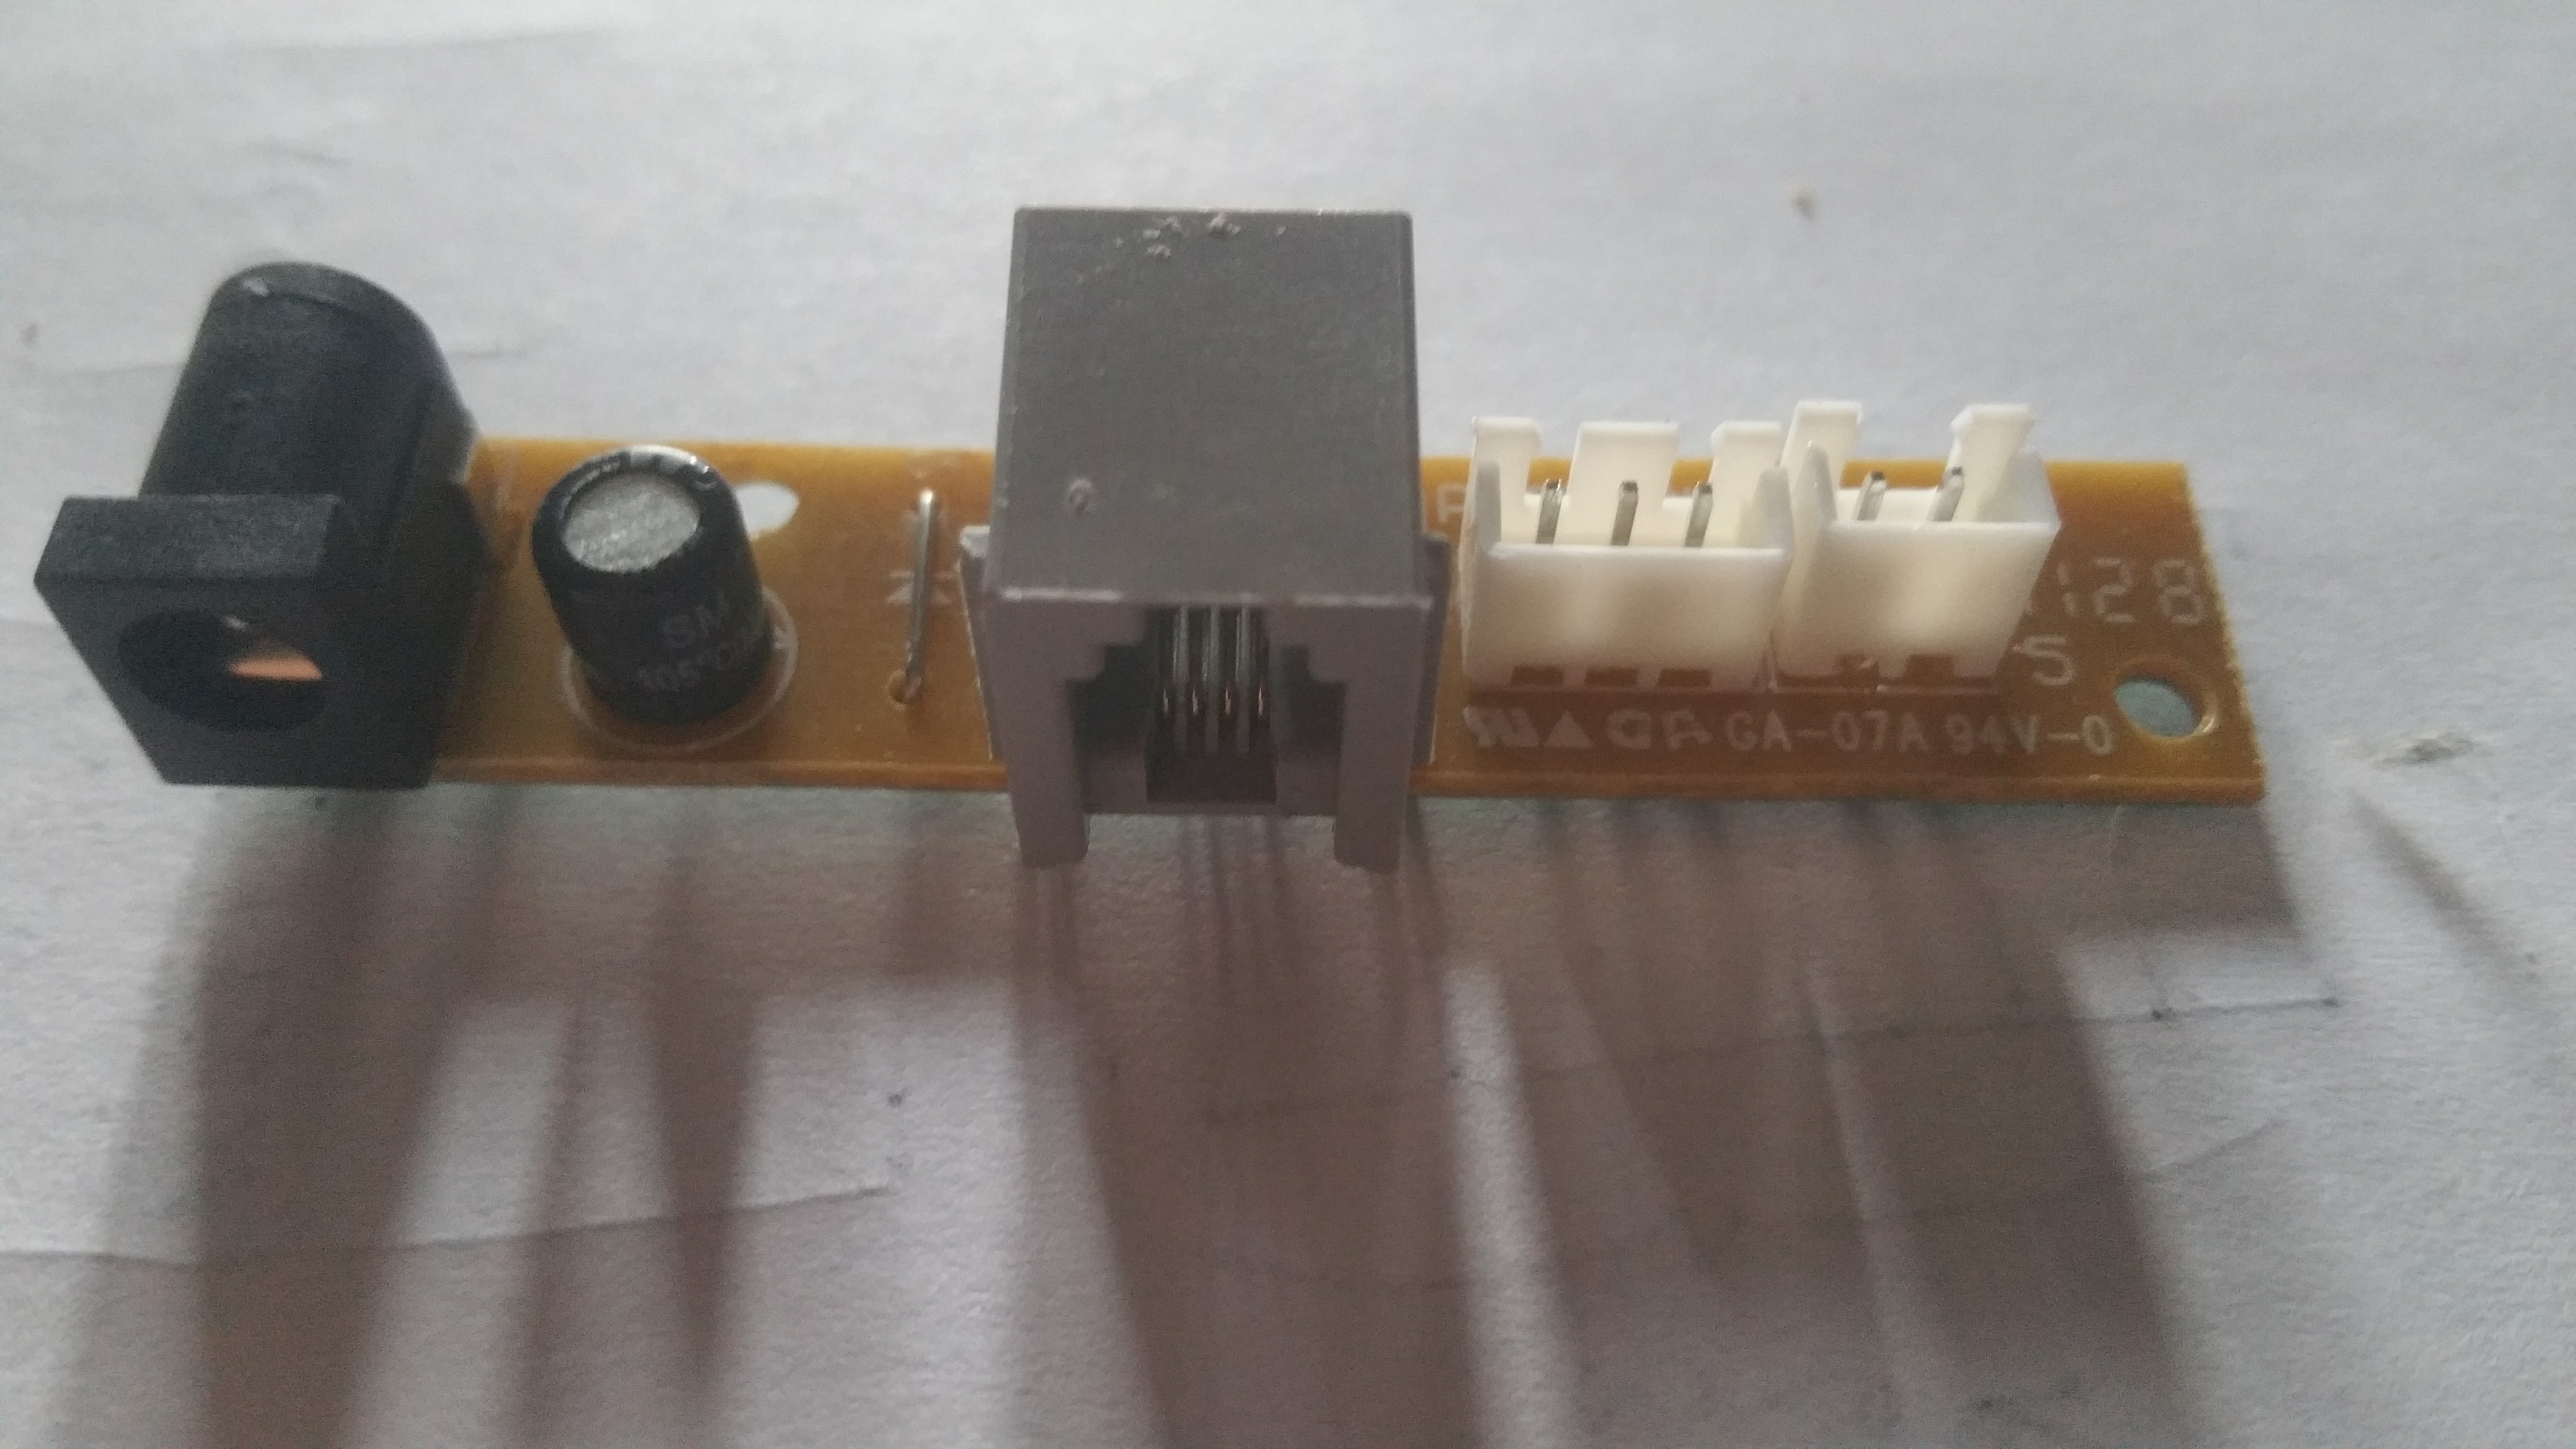
\includegraphics[width=0.5\textwidth]{img/img8.jpg}
  \caption{The secondary printed circuit board. This board connects the sensor to the 
  primary circuit board.}
  \label{fig:img8}
\end{figure}

\subsection{The Sensor}
A proximity sensor is connected to the secondary printed circuit board via a patch cable (pictured in Fig. \ref{fig:img10}). 
The sensor appears to be an ultrasonic sensor which works by emitting a pulse of human-inaudible sound and ``listening'' for
the pulse to return. 

\begin{figure}[h!]
  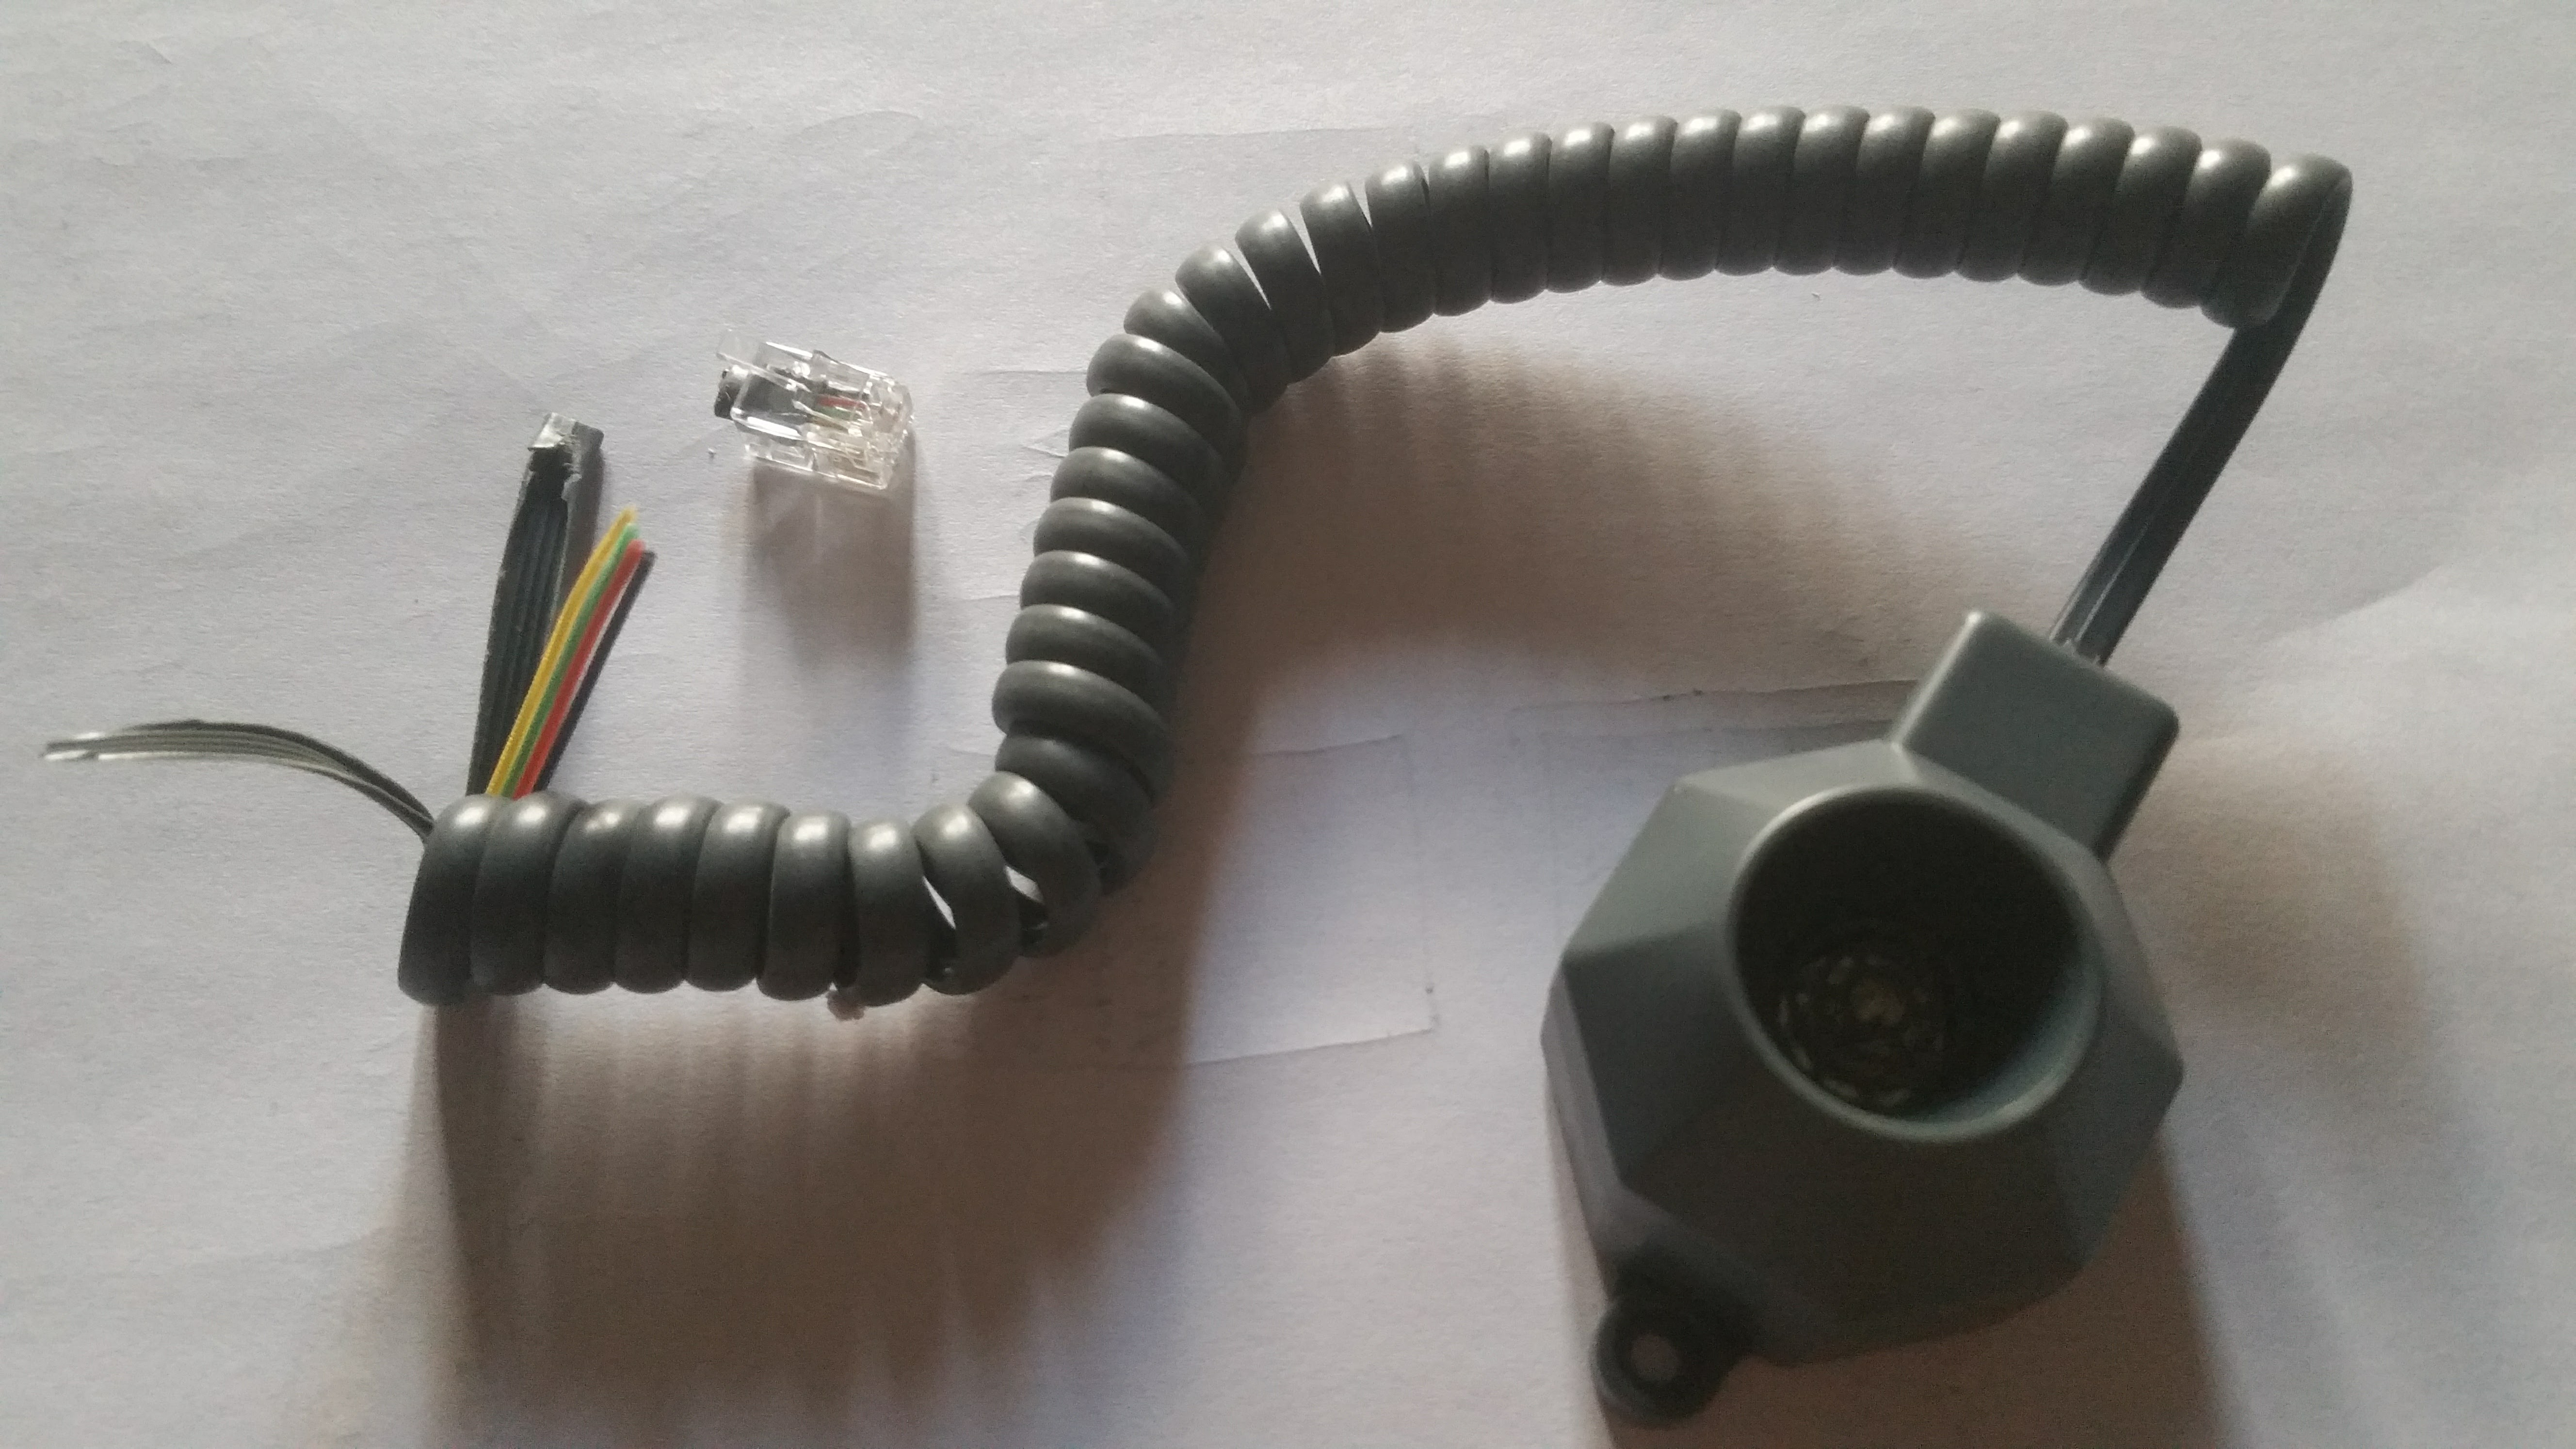
\includegraphics[width=0.5\textwidth]{img/img10.jpg}
  \caption{An ultrasonic sensor is connected to the secondary board via a patch cable -- shown here after having the end cut}
  \label{fig:img10}
\end{figure}
\FloatBarrier


\section{Conclusion}
The PEAK\textsuperscript{TM} PKCORJ GARAGE PARKING SENSOR is a simple and inexpensive device that provides an easy tear-down and contains a few salvageable parts. The ultrasonic sensor is a likely candidate for future use as is the battery bank that is
formed into the back half of the shell. Unfortunately, there seems to be very little in the way of documentation for this device, 
and attempts to find subsequent copies of this model have turned up very little.

\newpage

\appendix

\begin{figure}[h]
  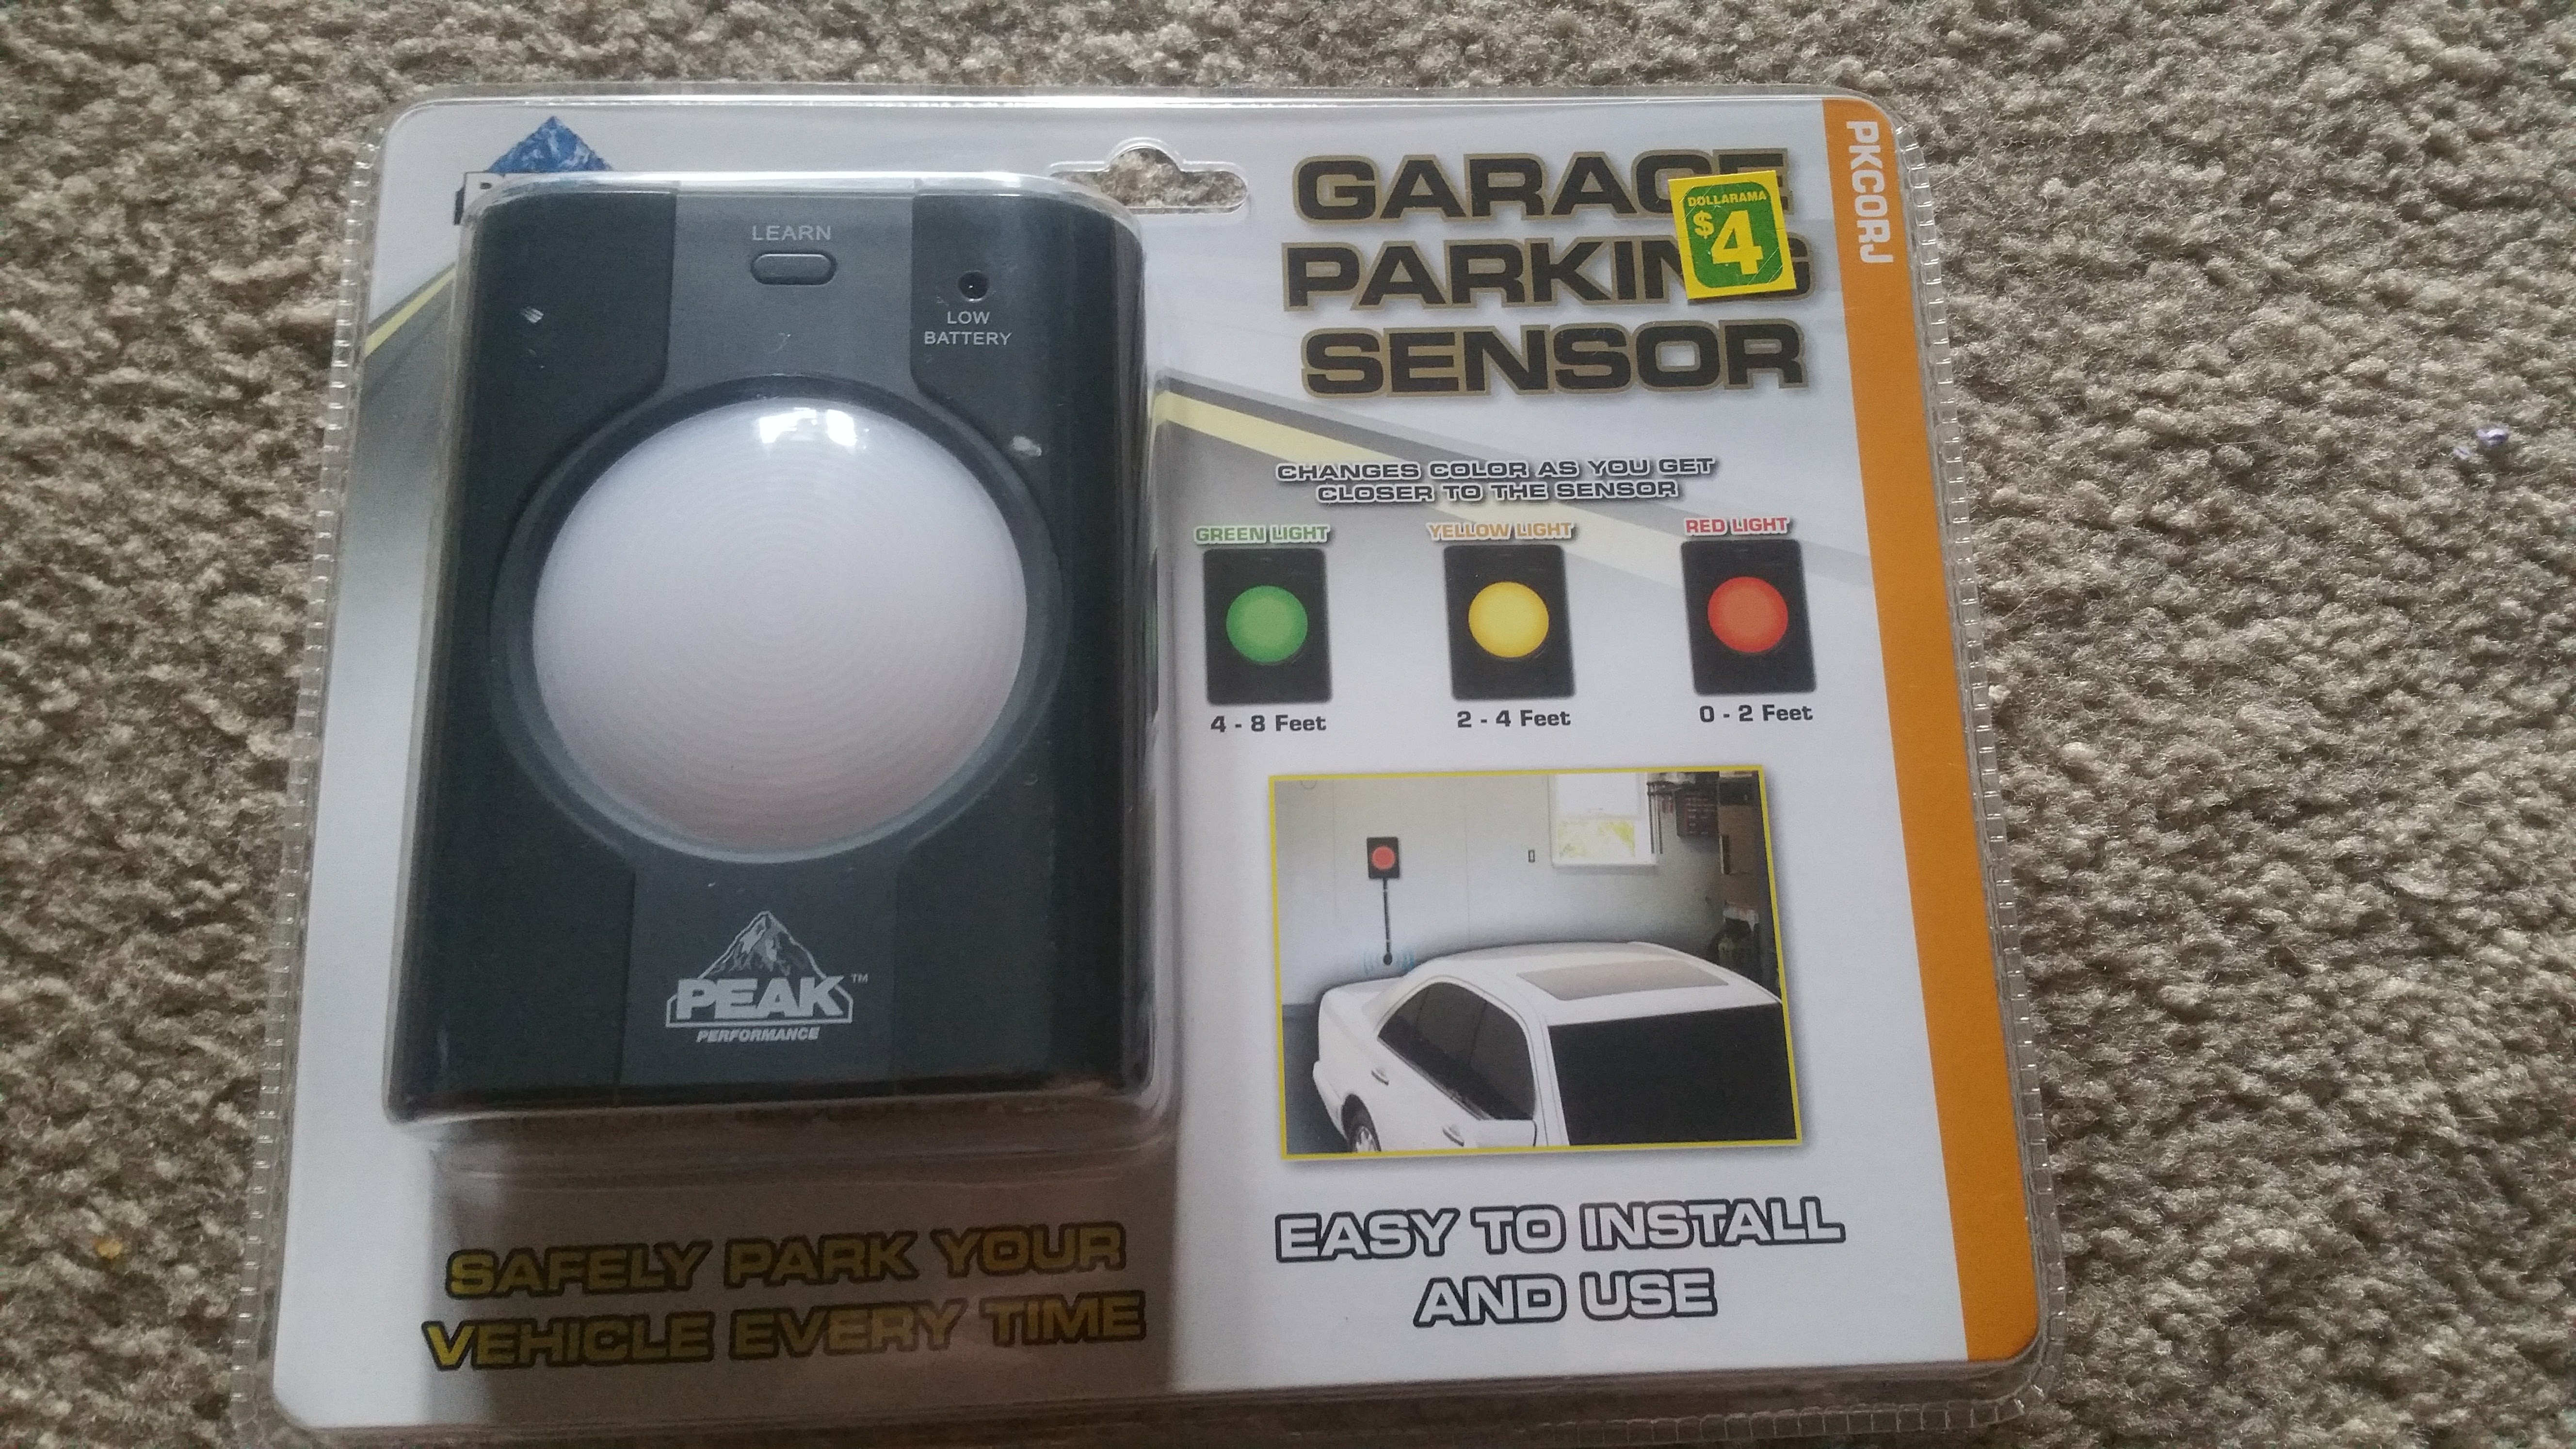
\includegraphics[width=0.5\textwidth]{img/img1.jpg}
  \caption{The front packaging of the  PEAK\textsuperscript{TM} PKCORJ GARAGE PARKING SENSOR}
  \label{fig:img1}
\end{figure}

\begin{figure}[h]
  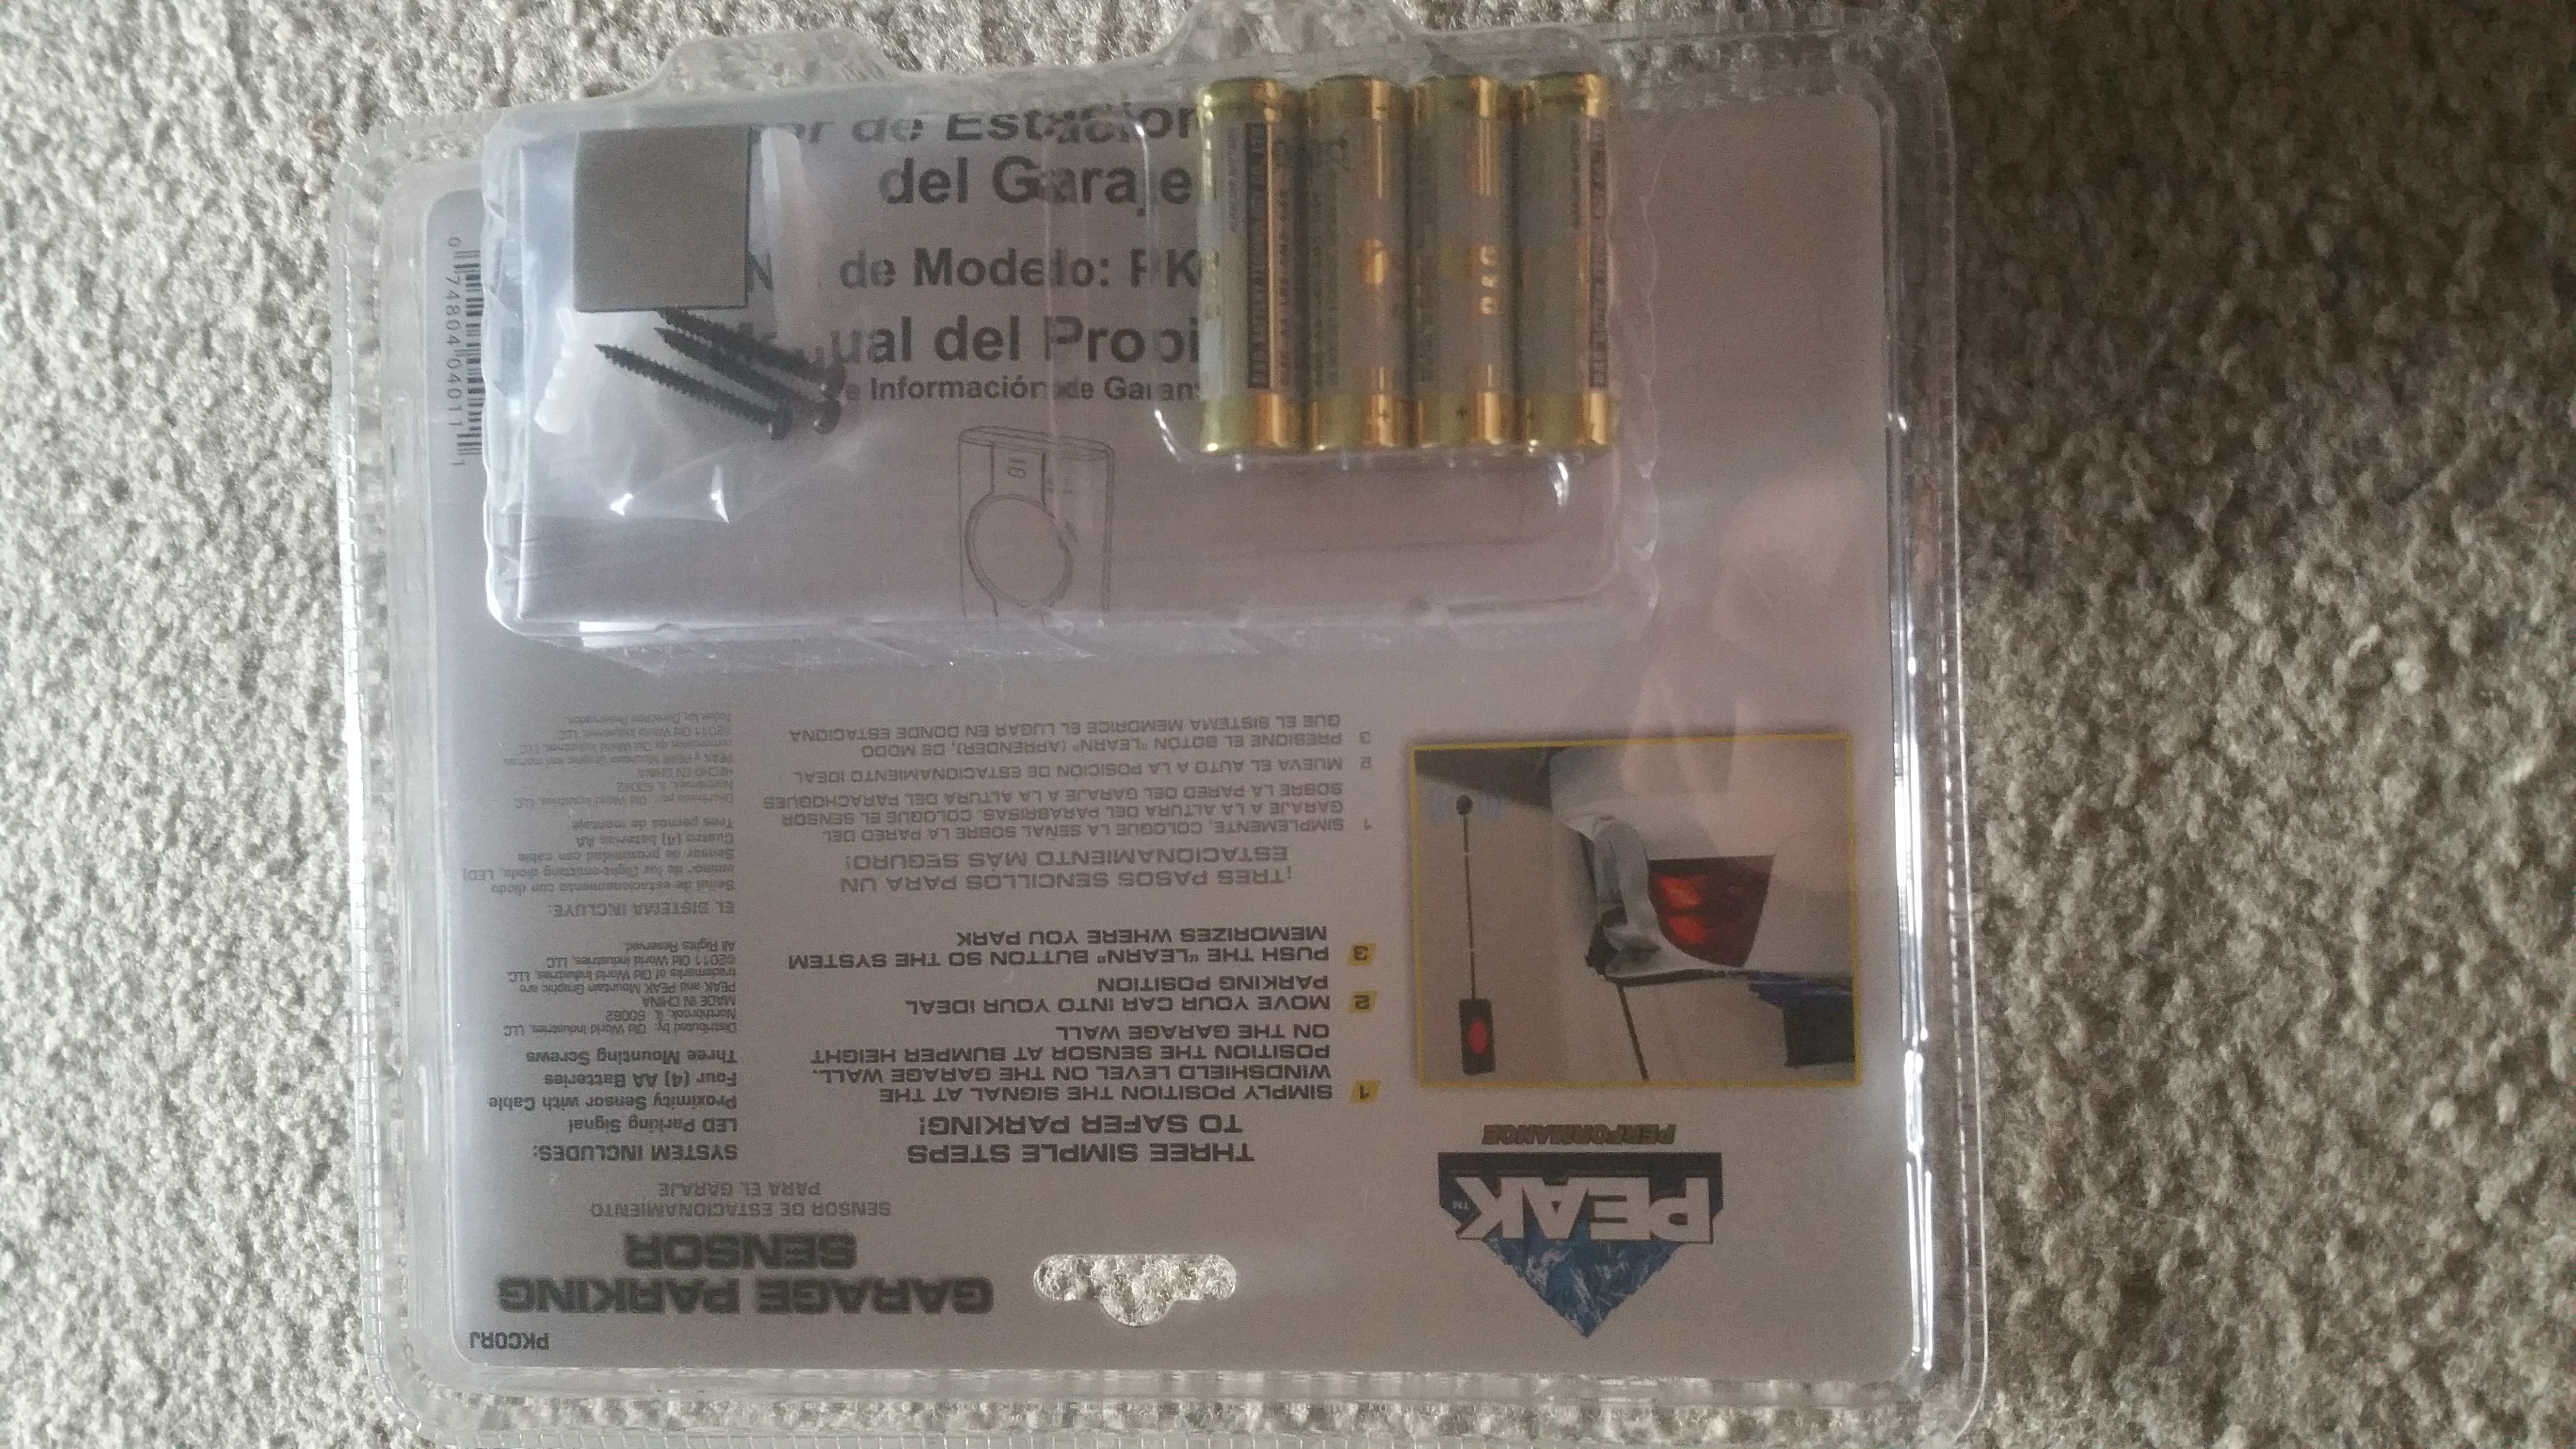
\includegraphics[width=0.5\textwidth, angle= 180,origin=c]{img/img2.jpg}
  \caption{The back packaging of the  PEAK\textsuperscript{TM} PKCORJ GARAGE PARKING SENSOR}
  \label{fig:img2}
\end{figure}

\begin{thebibliography}{1}

\bibitem{holtek:holtek}
HOLTEK SEMICONDUCTOR INC.(2009).HT46RS03/HT46RS03E/HT46RS03P/HT46RS03PE 2K 8-Bit OTP MCU with OPA \& Comparator.[online]\\ 
 Hsinchu, Taiwan: HOLTEK SEMICONDUCTOR INC. Available at:\\ 
 https://datasheetspdf.com/pdf/1064358/HoltekSemiconductor/HT46RS03PE/1 [Accessed 19 Jan. 2019].

\end{thebibliography}


% that's all folks
\end{document}


